\documentclass{article}

\usepackage{tikz}
\usetikzlibrary{shapes}

\usepackage{dirtree}
\usepackage{hyperref}
\usepackage{listings}
\usepackage{color}


\definecolor{codegreen}{rgb}{0,0.6,0}
\definecolor{codegray}{rgb}{0.5,0.5,0.5}
\definecolor{codepurple}{rgb}{0.58,0,0.82}
\definecolor{backcolour}{rgb}{0.95,0.95,0.92}
\definecolor{keywordcolour}{rgb}{0.0,0.0,0.92}
 
\lstdefinestyle{mystyle}{
    backgroundcolor=\color{backcolour},   
    commentstyle=\color{codegreen},
    keywordstyle=\color{keywordcolour},
    numberstyle=\tiny\color{codegray},
    stringstyle=\color{codepurple},
    basicstyle=\footnotesize,
    breakatwhitespace=false,         
    breaklines=true,                 
    captionpos=b,                    
    keepspaces=true,                 
    numbers=left,                    
    numbersep=5pt,                  
    showspaces=false,                
    showstringspaces=false,
    showtabs=false,                  
    tabsize=2
}

\lstset{style=mystyle}

\author{Marco Jakob}
\title{Kubernetes Full Stack Application}

\begin{document}

\maketitle
\newpage
\tableofcontents
\newpage

\section{Introduction}
This Introduction should give an end to end overview to deploy a sample Application with multiple Services and a Databases completely on Kubernetes.
The Application generates Random Numbers, saves them with a Timestamp on a database. Displays the new Number on a Frontend and also shows Graphs from previous Random Numbers based on their Producers Id.
The Goal of the whole application is first to create an end to end Application fully Cloud native which runs as well locally without any changes. The second goal is to show graphically the self healing process of Kubernetes, namely when we delete a random generator Pod, it should automatically create a new Random generator Pod with a new Id.
\subsection{Technology}
\begin{table}[h]
\begin{tabular}{ll}
\textbf{Service} & \textbf{Technology}  \\ \hline
Random Number Generator circle& Python Flask \\
Database to store previous Numbers & Mysql Database \\
Microservice for requesting new Numbers & Spring Boot Java \\
Microservice for gathering Statistics & Spring Boot Java \\
Frontend & Angular with Spring Boot \\
Routing Server & Nginx \\
Server OS & Ubuntu Server 18.5.1  LTS
\end{tabular}
\end{table}

All the Applications are Running inside of an own Docker Container and Managed within a Kubernetes Pod and accessible via a Kubernetes Service where only the Frontend Service is bound to a Node Port.
\subsection{Model}
The Following Picture should give an overview about the different Services and how they work with each other.

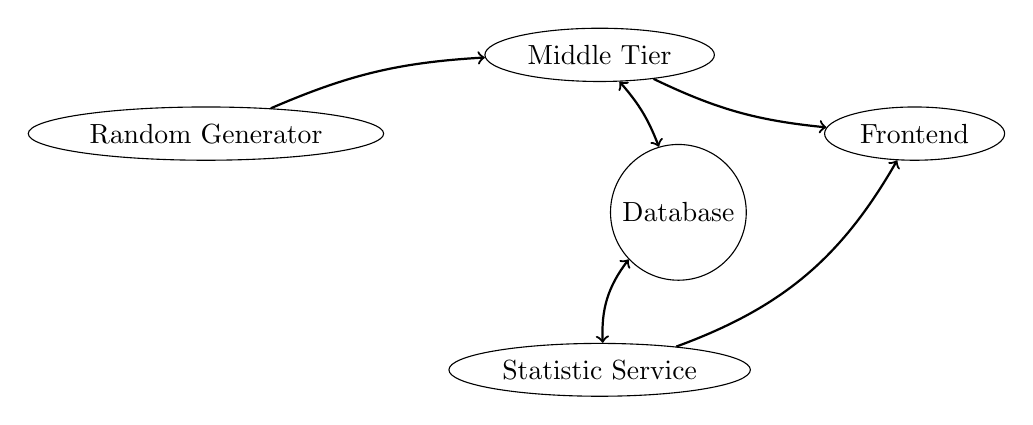
\begin{tikzpicture}
\node (A) at (0,0) [ellipse, draw] {Random Generator};
\node (B) at (5,-3) [ellipse, draw] {Statistic Service};
\node (C) at (6,-1) [circle, draw] {Database};
\node (D) at (9,0) [ellipse, draw] {Frontend};
\node (E) at (5,1) [ellipse, draw] {Middle Tier};

\draw[<->, thick] (B) to[bend left=20] (C);
\draw[->, thick] (B) to[bend right=20] (D);
\draw[->, thick] (A) to[bend left=10] (E);
\draw[->, thick] (E) to[bend right=10] (D); 
\draw[<->, thick] (E) to[bend left=10] (C);

\end{tikzpicture}

\section{Installing Kubernetes}

\section{Create Services}
\subsection{Database}
In the further sections we will use a plain mysql docker container as a database. In order to use the Application completely locally, a local mySQL database has to be installed and a schema for the random generator application needs to be provided for a specific randgenuser.
If there is not yet a local mySQL database installed it can be done with the following command:
\begin{lstlisting}[language=Bash]
sudo apt-get update
sudo apt-get install mysql-server
\end{lstlisting}
After the installation log in to MySQL as root. 
\begin{lstlisting}[language=Bash]
sudo mysql
\end{lstlisting}
Now the Database and the user can be created and permissions to the respective schema will be given.
\begin{lstlisting}[language=SQL]
CREATE database db_example;
CREATE USER 'springuser'@'localhost' IDENTIFIED BY ThePassword;
GRANT ALL PRIVILEGES ON *.db_example TO 'springuser'@'localhost';
\end{lstlisting}
With this, the Database is ready to used by the Random Generator Example from localhost.

\subsection{Random Generator}
The Random Generator will be a verry simple Python App which has an unique Id per Service instance. It will return his id and a new Random Number. For this application we create a folder called RandGen with the following Structure.

\dirtree{%
.1 RandGen.
.2 Dockerfile.
.2 rand\_gen.py.
.2 requirements.txt.
}
The Dockerfile is needed to create the Docker Image which will be used from Kubernetes to Create the Random Generator Service.
rand\_gen.py is the complete Random Generator Python application based on Flask\footnote{More information about Flask can be found on the official Homepage \url{http://flask.pocoo.org/}}.
 \lstinputlisting[language=Python]{Applikationen/generator/rand_gen.py}
In requirements.txt are the Python packages specified. In this case it is flask. therefore this file contains only one line which is
\begin{verbatim}
Flask==1.0.2
\end{verbatim}

The Dockerfile to create the Docker image:
\lstinputlisting[language=Bash]{Applikationen/generator/Dockerfile}



\subsection{Middle Tier}

The Middle Tier Application is created with Spring Initializer.
Unter the following link \url{https://start.spring.io/} Helps to bootstrap very fast a simple Spring Boot application.
In our case the fields should be filled out as followed:
\begin{tabbing}
\begin{tabular}{ll}
Project & Maven Project \\
Language & Java \\
Spring Boot & 2.1.3 (All versions would apply) \\
Group & ch.toky.randgen \\
Artifact & middletier \\
Name & MiddleTier \\
Description & Middle Tier Service for Random Generator Application \\
Packaging & Jar \\
Java Version & 8 \\
Dependencies & Web, JPA, MySQL, Rest Repositories
\end{tabular}
\end{tabbing}
The Website will create a zip file to download. This zipfile has to be extracted to the desired Project folder.
\dirtree{%
.1 middletier.
.2 Dockerfile.
.2 mvnw.
.2 mvnw.cmd.
.2 pom.xml.
.2 src.
}
all blue folders are already given. the Dockerfile still has to be created.

Now inside of the Project create the following Project Structure and files.

\dirtree{%
.1 ch.toky.randgen.middletier.
.2 MiddletierApplication.java.
.2 ch.toky.rand-gen.middle-tier.model.
.3 PodStat.java.
.3 RandomNumber.java.
.2 ch.toky.rand-gen.middle-tier.repository.
.3 PodStatRepository.java.
}
The file MiddleTierApplication.java should already be in place. as Spring Boot Initializr created this with the complete Folder structure. the packages controller, model and repository need to be created.
Inside of controller, A file named MiddletierController.java needs to be created with the following content.

Within the model package two new Files have to be created: PodStat.java and RandomNumber.java.

PodStat is an Entity and therefore the class has to be annotated with @Entity.
It contents the following fields with their respective getter and Setter Methods.
\begin{lstlisting}[language=Java]
@Id
@GeneratedValue(strategy=GenerationType.AUTO)
private Long podStatID;
private String id;
private Long timeStamp;
private Long counter;
\end{lstlisting}

The class RandomNumber is only a DTO which is retreived from the random generator Service. Therefore there is no need for a annotation.
Only the following Fields needs to be declared with their getters and setters:

\begin{lstlisting}[language=Java]
private String id;
private Long randNumber;
\end{lstlisting}

In the repository package the file PodStatRepository.java will be created.
As this java file is not a class but an interface it needs to be changed to interface and extends JpaRepository<PodStat, Long>
and it will be annotated with @Repository

Now those two methods are created 
\begin{lstlisting}[language=Java]
@Query("Select count(ps.id) from PodStat ps where ps.id = ?1")
Long countUniqueId(String id);

@Query("Select count(ps.id) from PodStat ps")
Long findMaxCount();
\end{lstlisting}

Witin the controller all the endpoints are declared. Therfore it will be annotaded with @RestController

Those fields are needed within the controller and are therefore declared first.
\begin{lstlisting}[language=Java]
@Autowired
private ObjectMapper objectMapper;
@Autowired
private PodStatRepository podStatRepository;
private Map<String, String> env = System.getenv();
\end{lstlisting}
As there should not be any hardcoded url according to the 12 Factor application \footnote{Accessible at \url{https://12factor.net/}}, the Url will be retreived through a System Variable.

Now a controller Method with the business logic can be declared:
\begin{lstlisting}[language=Java]
@RequestMapping(value = "/", produces = "application/json")
public RandomNumber getRandom() {

    RandomNumber randNum = getNewRandomNumber();
    Long maxCountId = podStatRepository.countUniqueId(randNum.getId());
    Long maxCountOverall = podStatRepository.findMaxCount();
    PodStat tmpPod = new PodStat();
    tmpPod.setId(randNum.getId());
    tmpPod.setTimeStamp(maxCountOverall+1);
    tmpPod.setCounter(maxCountId +1);
    podStatRepository.save(tmpPod);

    return randNum;

}
\end{lstlisting}
The above Method listens on the path / and returns the Random number after saving it to the database with the actual count.

Now the last Method is used to retreive the Random Number from the Random Generator Service.
\begin{lstlisting}[language=Java]
private RandomNumber getNewRandomNumber() {

    String randGenUrl=env.get("RANDOM_GENERATOR_URL");
    String URL = randGenUrl;
    RestTemplate restTemplate = new RestTemplate();

    return   restTemplate.getForObject(URL, RandomNumber.class);

}
\end{lstlisting}
Above Source code contains the Controller and the Service, which should be separated optimally.
Next two files represents POJOs which are going to be used from controller and provided by Repositories.

The last thing which needs to be done for the Middle Tier Service is to setup the default values for the Database Connection.
\begin{lstlisting}
spring.jpa.hibernate.ddl-auto=update
spring.datasource.username=random_user
spring.datasource.password=random_password
spring.datasource.url=jdbc:mysql://localhost:3306/rand_numbers
\end{lstlisting}
The datasource configurations are going to be overwritten by Environment Variables once they run inside of a Docker Container.




\subsection{Statistic Service}
The Statistic Service has the same setup as the Middle Tier client.
Therefore the Project will be created too with Spring Boot initializer.
\begin{tabbing}
\begin{tabular}{ll}
Project & Maven Project \\
Language & Java \\
Spring Boot & 2.1.3 (All versions would apply) \\
Group & ch.toky.randgen \\
Artifact & stattier \\
Name & Stattier \\
Description & Statistic Tier Client for Random Generator Application \\
Packaging & Jar \\
Java Version & 8 \\
Dependencies & Web, JPA, MySQL, Rest Repositories
\end{tabular}
\end{tabbing}

For the statistic Tier Service we need to create the following Package structure:
\dirtree{%
.1 ch.toky.randgen.statservice.
.2 StatserviceApplication.java.
.2 ch.toky.randgen.statservice.controller.
.3 Controller.java.
.2 ch.toky.randgen.statservice.model.
.3 PodStat.java.
.3 Series.java.
.3 SeriesItem.java.
.3 Stat.java.
.2 ch.toky.randgen.statservice.repository.
.3 PodStatRepository.java.
.2 ch.toky.randgen.statservice.service.
.3 StatService.java.
}

For this time, we will leave the Main Class allone in the file StatserviceApplication.java. Which means we do not have to change this file as Spring Boot already did everything needed for us.

Controller.java will be annotated with @RestController as it contains all our endpoints.

next, we need the StatService class in this controller, this is why we inject it with @Autowired.
\begin{lstlisting}[language=Java]
@Autowired
StatService statService;
\end{lstlisting}

Now we can also create our two endpoints, one for all stats, and one with the history.

\begin{lstlisting}[language=Java]
@RequestMapping(method = RequestMethod.GET, value="/")
public List<Stat> getAllPodStats(){

    return statService.getAllPodStats();
}
    
    
@RequestMapping(method = RequestMethod.GET, value="/history")
public List<Series> getAllPodStatsHistory(){
        
	return statService.getPodHistory();	
}
\end{lstlisting}

We could leave the method out as GET is anyway the default method but we leave it here for for the understanding.

next we are going to declare all our Entities.

All of them are annotated with @Entity.
For simplicity i will only show all fields but of cource also the getter and setter methods needs to be implemented.

Fields for PodStat:

\begin{lstlisting}[language=Java]
@Id
@GeneratedValue(strategy=GenerationType.AUTO)
private Long podStatID;
private String id;
private Long timeStamp;
private Long counter;
...
\end{lstlisting}

Series not annotated with @Entity as it is only a helper Entity we have also a contructor in order to initialize a new Array List.
\begin{lstlisting}[language=Java]
private String name;
private List<SeriesItem> series;
public Series(String name) {
	super();
	this.name = name;
	this.series = new ArrayList<SeriesItem>();
}
...

public void appendSeries(SeriesItem seriesItem){
    this.series.add(seriesItem);
}
\end{lstlisting}

SeriesImtem is the second helper class we are going to use and therefore as well not annotated with @Entity
\begin{lstlisting}[language=Java]
private Long name;
private Long value;
	
public SeriesItem(Long name, Long value) {
	super();
	this.name = name;
	this.value = value;
}
\end{lstlisting}


\begin{lstlisting}[language=Java]
private String id;
private Long counter;

public Stat(String id, Long counter) {
	super();
	this.id = id;
	this.counter = counter;
}
\end{lstlisting}

Now we can implement the Repository (annotated with @Repository) as an interface which extends JpaRepository<PodStat, String>

\begin{lstlisting}[language=Java]
@Query("Select count(ps.id) from PodStat ps where ps.id = ?1")
Long countUniqueId(String id);
	
@Query("Select distinct ps.id from PodStat ps")
List<String> findUniqueIds();
	
@Query("Select ps from PodStat ps where ps.id = ?1")
List<PodStat> findByIds(String id);
\end{lstlisting}

Now the last file is the most important one as there we will have all the business logig in it.

We need to annotate it with @Service in order to make it available for Spring Boot to create a Bean out of it.


\begin{lstlisting}[language=Java]
@Autowired
PodStatRepository podStatRepository;

private Iterable<String> getAllIds() {
	Iterable<String> source = podStatRepository.findUniqueIds();
	return source;
}

public List<Stat> getAllPodStats() {

	Iterable<String> source = getAllIds();
	List<Stat> podStatistics = new ArrayList<Stat>();
	source.forEach((id) -> {
		podStatistics.add(new Stat(id, podStatRepository.countUniqueId(id)));
	});
	return podStatistics;
}
	
public List<Series> getPodHistory(){
		
	Iterable<PodStat> source = podStatRepository.findAll();	
	Map<String, Series> podHistorys = new HashMap<>();	
	source.forEach( (entry) -> {				
		if(podHistorys.get(entry.getId()) == null) {			
			podHistorys.put(entry.getId(), new Series(entry.getId()));			
		}
		podHistorys.get(entry.getId())
		.appendSeriesItem(new SeriesItem(entry.getTimeStamp(), entry.getCounter()));							
	});
		
	List<Series> plainSeries = new ArrayList<>(podHistorys.values());
	return plainSeries;	
}
\end{lstlisting}

Now that all the java fils are created we can also create the Dockerfile for this Service.

\lstinputlisting[language=Bash]{Applikationen/statservice/Dockerfile}

Basically the Dockerfile for this Service looks pretty much the same as the one for the Middle tier except that we do not need to declare an environment variable for the random generator.


\subsection{Frontend}
The frontend Application is build with Spring Boot and 

Creating Spring Boot Application:
\begin{tabbing}
\begin{tabular}{ll}
Project & Maven Project \\
Language & Java \\
Spring Boot & 2.1.3 (All versions would apply) \\
Group & ch.toky.randgen \\
Artifact & frontend \\
Name & Frontend \\
Description & Frontend Service \\
Packaging & Jar \\
Java Version & 8 \\
Dependencies & Web, Rest Repositories
\end{tabular}
\end{tabbing}



\section{Deploy Services to Kubernetes}

\end{document}